\documentclass{article}

% ==================================================
% FONT
% ==================================================

\usepackage{newtxtext}
\usepackage{newtxmath}

% ==================================================
% TIKZ
% ==================================================

\usepackage{tikz}
\usetikzlibrary{arrows.meta}

% ==================================================
% COLORS
% ==================================================

\definecolor{navy}{RGB}{20,55,100}
\definecolor{blue}{RGB}{40,90,150}
\definecolor{bluepale}{RGB}{235,242,250}

\definecolor{gold}{RGB}{190,140,40}
\definecolor{goldpale}{RGB}{255,248,220}

\definecolor{green}{RGB}{45,140,85}
\definecolor{greenpale}{RGB}{230,248,238}

% ==================================================
% DOCUMENT
% ==================================================

\begin{document}
	
	\begin{figure}[ht]
		\centering
		
		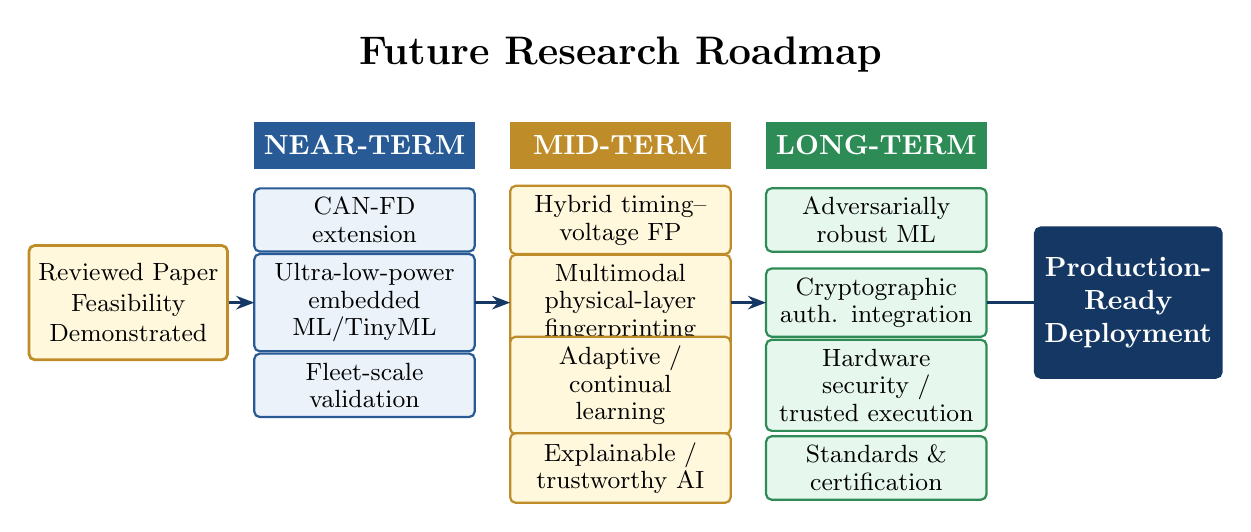
\begin{tikzpicture}[x=1cm,y=1cm]
			
			% ==================================================
			% FIGURE HEADING
			% ==================================================
			
			\node[
			align=center,
			font=\bfseries\fontsize{14}{17}\selectfont
			] at (6.25,3.15)
			{Future Research Roadmap};
			
			% ==================================================
			% REVIEWED PAPER
			% ==================================================
			
			\node[
			rectangle,
			rounded corners=2pt,
			draw=gold,
			fill=goldpale,
			line width=1pt,
			minimum width=1.7cm,
			minimum height=1.45cm,
			align=center,
			font=\fontsize{9}{11}\selectfont
			] (start) at (0,0)
			{Reviewed Paper\\
				Feasibility\\
				Demonstrated};
			
			% ==================================================
			% HEADERS
			% ==================================================
			
			\node[
			rectangle,
			fill=blue,
			text=white,
			minimum width=2.8cm,
			minimum height=0.6cm,
			align=center,
			font=\bfseries\fontsize{10}{12}\selectfont
			] at (3.0,2.0)
			{NEAR-TERM};
			
			\node[
			rectangle,
			fill=gold,
			text=white,
			minimum width=2.8cm,
			minimum height=0.6cm,
			align=center,
			font=\bfseries\fontsize{10}{12}\selectfont
			] at (6.25,2.0)
			{MID-TERM};
			
			\node[
			rectangle,
			fill=green,
			text=white,
			minimum width=2.8cm,
			minimum height=0.6cm,
			align=center,
			font=\bfseries\fontsize{10}{12}\selectfont
			] at (9.5,2.0)
			{LONG-TERM};
			
			% ==================================================
			% NEAR-TERM ITEMS
			% ==================================================
			
			\node[
			rectangle,
			rounded corners=2pt,
			draw=blue,
			fill=bluepale,
			line width=0.8pt,
			minimum width=2.8cm,
			minimum height=0.7cm,
			text width=2.55cm,
			align=center,
			font=\fontsize{9}{10}\selectfont
			] at (3.0,1.05)
			{CAN-FD extension};
			
			\node[
			rectangle,
			rounded corners=2pt,
			draw=blue,
			fill=bluepale,
			line width=0.8pt,
			minimum width=2.8cm,
			minimum height=0.7cm,
			text width=2.55cm,
			align=center,
			font=\fontsize{9}{10}\selectfont
			] at (3.0,0)
			{Ultra-low-power\\embedded ML/TinyML};
			
			\node[
			rectangle,
			rounded corners=2pt,
			draw=blue,
			fill=bluepale,
			line width=0.8pt,
			minimum width=2.8cm,
			minimum height=0.7cm,
			text width=2.55cm,
			align=center,
			font=\fontsize{9}{10}\selectfont
			] at (3.0,-1.05)
			{Fleet-scale\\validation};
			
			% ==================================================
			% MID-TERM ITEMS
			% ==================================================
			
			\node[
			rectangle,
			rounded corners=2pt,
			draw=gold,
			fill=goldpale,
			line width=0.8pt,
			minimum width=2.8cm,
			minimum height=0.7cm,
			text width=2.55cm,
			align=center,
			font=\fontsize{9}{10}\selectfont
			] at (6.25,1.05)
			{Hybrid timing--\\voltage FP};
			
			\node[
			rectangle,
			rounded corners=2pt,
			draw=gold,
			fill=goldpale,
			line width=0.8pt,
			minimum width=2.8cm,
			minimum height=0.7cm,
			text width=2.55cm,
			align=center,
			font=\fontsize{9}{10}\selectfont
			] at (6.25,0)
			{Multimodal physical-layer\\fingerprinting};
			
			\node[
			rectangle,
			rounded corners=2pt,
			draw=gold,
			fill=goldpale,
			line width=0.8pt,
			minimum width=2.8cm,
			minimum height=0.7cm,
			text width=2.55cm,
			align=center,
			font=\fontsize{9}{10}\selectfont
			] at (6.25,-1.05)
			{Adaptive / continual\\learning};
			
			\node[
			rectangle,
			rounded corners=2pt,
			draw=gold,
			fill=goldpale,
			line width=0.8pt,
			minimum width=2.8cm,
			minimum height=0.7cm,
			text width=2.55cm,
			align=center,
			font=\fontsize{9}{10}\selectfont
			] at (6.25,-2.10)
			{Explainable /\\trustworthy AI};
			
			% ==================================================
			% LONG-TERM ITEMS
			% ==================================================
			
			\node[
			rectangle,
			rounded corners=2pt,
			draw=green,
			fill=greenpale,
			line width=0.8pt,
			minimum width=2.8cm,
			minimum height=0.7cm,
			text width=2.55cm,
			align=center,
			font=\fontsize{9}{10}\selectfont
			] at (9.5,1.05)
			{Adversarially\\robust ML};
			
			\node[
			rectangle,
			rounded corners=2pt,
			draw=green,
			fill=greenpale,
			line width=0.8pt,
			minimum width=2.8cm,
			minimum height=0.7cm,
			text width=2.55cm,
			align=center,
			font=\fontsize{9}{10}\selectfont
			] at (9.5,0)
			{Cryptographic\\auth. integration};
			
			\node[
			rectangle,
			rounded corners=2pt,
			draw=green,
			fill=greenpale,
			line width=0.8pt,
			minimum width=2.8cm,
			minimum height=0.7cm,
			text width=2.55cm,
			align=center,
			font=\fontsize{9}{10}\selectfont
			] at (9.5,-1.05)
			{Hardware security /\\trusted execution};
			
			\node[
			rectangle,
			rounded corners=2pt,
			draw=green,
			fill=greenpale,
			line width=0.8pt,
			minimum width=2.8cm,
			minimum height=0.7cm,
			text width=2.55cm,
			align=center,
			font=\fontsize{9}{10}\selectfont
			] at (9.5,-2.10)
			{Standards \&\\certification};
			
			% ==================================================
			% PRODUCTION-READY DEPLOYMENT
			% ==================================================
			
			\node[
			rectangle,
			rounded corners=2pt,
			draw=navy,
			fill=navy,
			text=white,
			line width=1pt,
			minimum width=1.8cm,
			minimum height=1.9cm,
			align=center,
			font=\bfseries\fontsize{10}{12}\selectfont
			] (final) at (12.7,0)
			{Production-\\
				Ready\\
				Deployment};
			
			% ==================================================
			% ARROWS
			% ==================================================
			
			% Reviewed Paper -> Near-Term
			\draw[
			-{Stealth[length=2.3mm]},
			draw=navy,
			line width=0.9pt
			] (start.east) -- (1.6,0);
			
			% Near-Term -> Mid-Term
			\draw[
			-{Stealth[length=2.3mm]},
			draw=navy,
			line width=0.9pt
			] (4.4,0) -- (4.85,0);
			
			% Mid-Term -> Long-Term
			\draw[
			-{Stealth[length=2.3mm]},
			draw=navy,
			line width=0.9pt
			] (7.65,0) -- (8.1,0);
			
			% Long-Term -> Production
			\draw[
			-{Stealth[length=2.3mm]},
			draw=navy,
			line width=0.9pt
			] (10.9,0) -- (11.75,0);
			
		\end{tikzpicture}
		
	\end{figure}
	
\end{document}